In \sh, a session represents a complete working space of a user. It references a dataset consisting of molecules and a corresponding scaffold tree. The molecules of a session can be filtered to reduce the molecule count to a manageable size.

\begin{figure}[h]
   \centering
   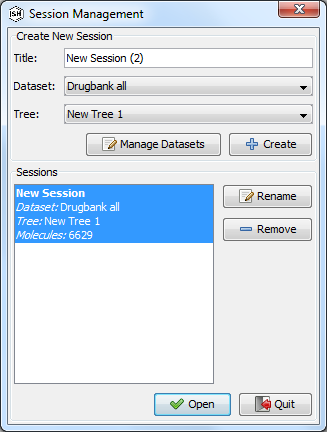
\includegraphics[scale=0.8]{images/sh_session_dialog.png}
   \caption{Session Management Dialog}
   \label{fig:session_dialog}
\end{figure}

The \guidialog{Session Management Dialog} shown in \figref{fig:session_dialog} appears after logging in, or by selecting \gui{Session $\rightarrow$ Load / Create} from the menu. If \gui{Open last used session} was selected in the \guidialog{Start Dialog}, the session management window does not appear and the last used session is opened instead. The session management consists of two areas. The upper area is used for creating new sessions. The lower area shows a list of available sessions and options for them. At the first start the session list will be empty, and a new session has to be created in order to start \sh.

To create a new session, choose a title, the dataset to create the session on, and the scaffold tree. The title can be changed later. After clicking on the \gui{Create} button, a filter dialog will appear, allowing to filter the selected dataset. The created session will then be displayed in the list of sessions in the lower area. To create a new dataset or to add a new tree to a dataset, click \gui{Manage Datasets}.

In the lower area of the session management window, the available sessions are shown with their title, dataset, tree and molecule count. Here the sessions can be renamed or removed, if they are no longer needed. To open a session, select the desired session and click the \gui{Open} button. Initially the last used session is selected in the list.

\hintbox{Important}{If you are running into database exceptions while saving a session of a larger dataset, this might be a problem with the maximum package size of \mysql. Please refer to \secref{sec:mysql_max_package_size} for further instructions about how to configure the \mysql server.}